\documentclass[parskip=full]{scrartcl}
\usepackage[utf8]{inputenc} % use utf8 file encoding for TeX sources
\usepackage[T1]{fontenc}    % avoid garbled Unicode text in pdf
\usepackage[english]{babel}  % english hyphenation, quotes, etc
\usepackage[colorlinks=true,linkcolor=blue]{hyperref}       % detailed hyperlink/pdf configuration
\usepackage{graphicx}       % provides commands for including figures
\usepackage{csquotes}       % provides \enquote{} macro for "quotes"
\usepackage{enumitem}
\usepackage{multicol}
\setlength{\columnsep}{4cm}
%\usepackage{lscape}	% provides landscape portrait

\usepackage{pdflscape}	% provides horizental landscape portrait


\usepackage{pdfpages}	% add another pdf in  Latex

\usepackage{tikz}


\usepackage{verbatim}	% provides multi-line comments

\usepackage{afterpage}
\usepackage{ragged2e}
\usepackage[export]{adjustbox}
\newcommand\tab[1][1cm]{\hspace*{#1}}


\title{\Huge \textbf{HePICS Test-Phase Document}}
\date{\today \vspace{+10ex}}
\author{Andres Stober \\
	\and Mehyar Cherni \\
	\and Ibrahim Bouriga \\ 
	\and Linjuan Fan \\
	\and Bahaa Mahjane \\ }

\begin{document}

\maketitle
\thispagestyle{empty}

\begin{tikzpicture}[remember picture, overlay]
  \node [anchor=north west, inner sep=0.5pt, yshift=-20pt,xshift=20pt]  at (current page.north west)
     {
\includegraphics[height=1.9cm]{Logo_KIT}};
\end{tikzpicture}

\begin{figure}[b]
\centering
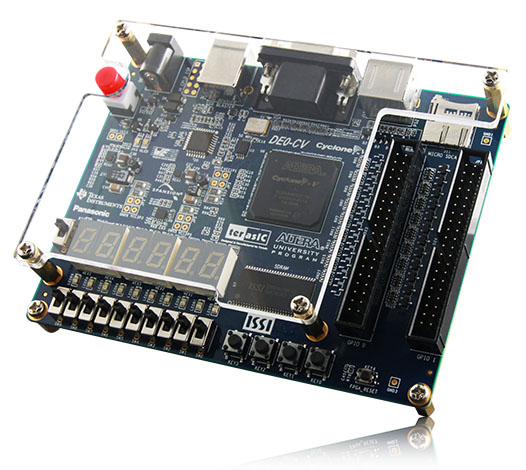
\includegraphics[width=0.45\textwidth, center]{boardimage}
\end{figure}

\pagebreak

\tableofcontents
\thispagestyle{empty}
\pagebreak



\section {Introduction}
For the purpose of testing submodules and base classes of our program, we configured GoogleTest on eclipse. As more tests were run, it turned out that the integration of the submodules was of a bigger difficulty than estimated, which is why we decided to re-structure the program, in a way we can use the old code, and make the integration of different parts an easier and safer process at the same time.\\
We oriented ourselves as much as possible to the design set during the design phase, and of course, with minor changes, our goal has been mostly achieved, since unit tests are all successful.\\
As much as this is seen as an achievment, it is safe to say and keep in mind that tests are run to uncover errors, not to prove their absence. Therefore, the effectiveness of these tests will be proven in the next phase, when the full integration is finished.
\section {Google Test}
Google Test is a unit testing library for the C++ programming language, based on the xUnit architecture. This section describes reasons why we decided to use this framework.
\begin{itemize}
	\item  Google Test is designed to be portable and it works around various bugs in various compilers and environments
	\item  Google's test framework has built-in assertions that are deployable in software where exception handling is disabled
	\item  Running the tests is simple and it’s easy to write assertions that generate informative messages
	\item  Google Test automatically detects your tests and doesn’t require you to enumerate them in order to run them.
	\item  Google's test framework provides excellent support for handling such situations. You can repeat the same test as many times as neededs using the Google framework. See \ref{fig:google_test} 
	
\begin{figure}[h]
	\centering
	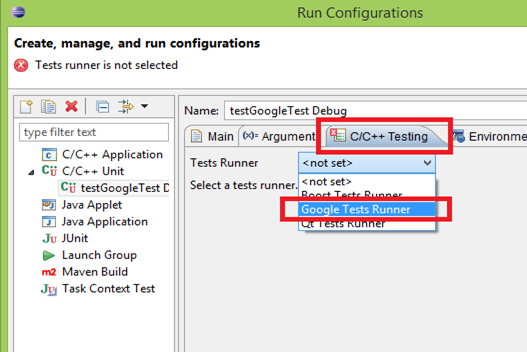
\includegraphics[width=0.75\textwidth]{google_test}
	\caption{google test}
	\label{fig:google_test}
\end{figure}

\end{itemize}
\pagebreak
\section {Tests}
The following displays the tests that were run, and their results.
\pagebreak
\subsection{Network}
The network consists of a vector of multiple of layers, many of which were tested. The activation layers were not tested as they are simple mathematic functions. Example : relu, sigmoid
\subsubsection{Network}
The constructor of Network loads the layers from a configuration file through Caffe parser. Therefore, tests were run to check if these layers are properly loaded in the class. See figure \ref{fig:network_test} % insert here screenshot of test code

\begin{figure}[h]
		\centering
		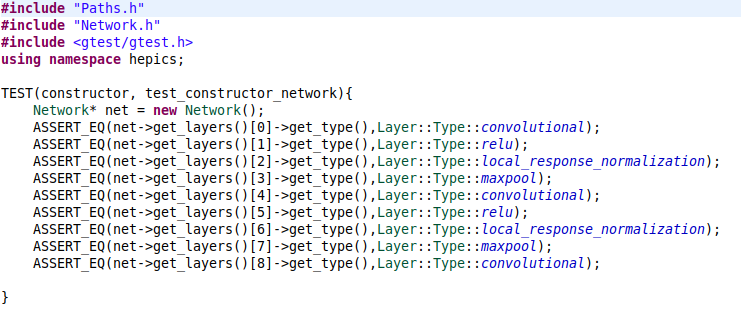
\includegraphics[width=1\textwidth]{network_test}
		\caption{network test}
		\label{fig:network_test}
\end{figure}

\subsubsection{Caffe}
Caffe was used to access functions which made the network model easier to implement, since it offers parsing methods to fill each layer with its proper fields. It also provided as the weights. See \ref{fig:caffe} % insert here screenshot of test code

\begin{figure}[h]
		\centering
		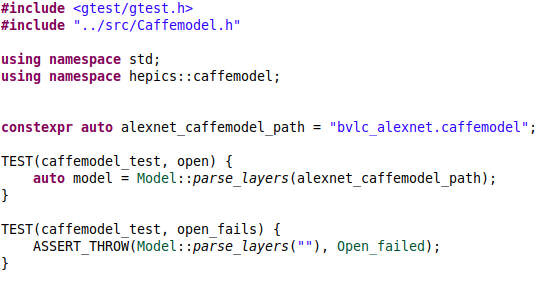
\includegraphics[width=0.75\textwidth]{caffe_test}
		\caption{caffe test}
		\label{fig:caffe_test}
\end{figure}

\subsubsection{Convolutional Layer}
The convolutional layer has one of the most complicated implementations of the network model. 4 test cases were run to make sure it is running the way it should.

	\textbf {Convolution}
	\tab  The idea of the convolution is to go through all image pixels and use the filter on them. However the filter might not cover the right pixels that's why we need to check in every iteration if the latter is within the image. Other important things to be considered in this procedure. For instance the caffe model of the layer itself, which provide further specification other than usual channels, height and width.
	
	\textbf {ReLU}
	\tab The caffe model suggest also that the activation function should be considered as a layer too. In order to achieve this approach, we just pass the output of the convolutional as an input for this layer. The function will be applied on the image data and the dimensions of the output do not changes.

	\textbf {Test}
	\tab In order to avoid any unexpected behaviour of the convolutional layer we apply different filters with diffrerent strides on the input. Differents paddings were also used by the input. However we model the image as a set of data and do not use real images
in this approach, so that we can avoid interpreting graphical representation by the output. The data are represented as vectors of float. The expected output are calculated manually and compared to the one produced by the layer. See \ref{fig:convolution_test} % insert here screenshot of test code

\begin{figure}[h]
		\centering
		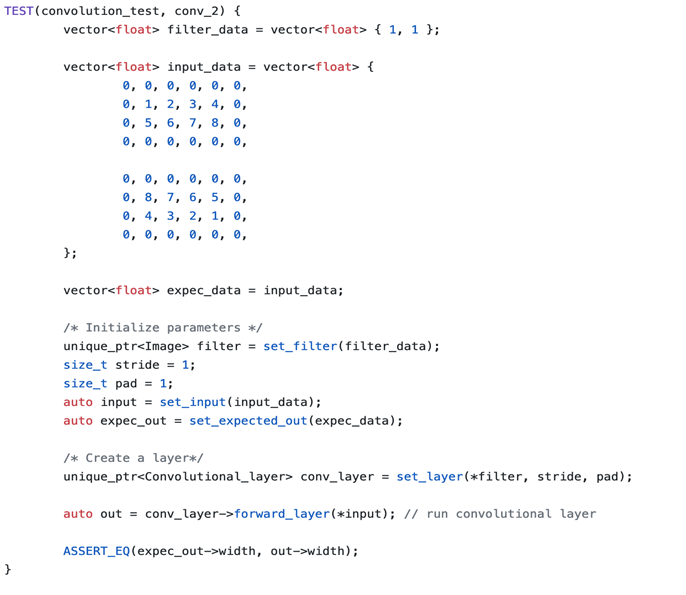
\includegraphics[width=1\textwidth]{convolution_test}
		\caption{convolution test}
		\label{fig:convolution_test}
\end{figure}

\subsubsection{Maxpool Layer}
Its function is to progressively reduce the spatial size of the representation to reduce the amount of parameters and computation in the network, and hence to also control overfitting. See \ref{fig:maxpool_test} % insert here screenshot of test code

\begin{figure}[h]
		\centering
		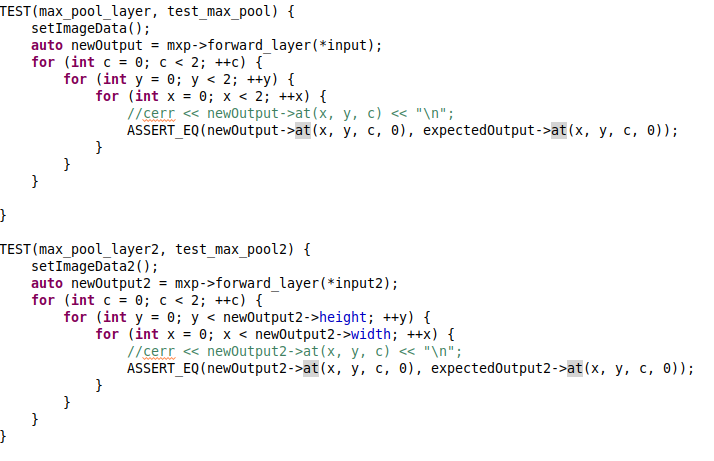
\includegraphics[width=1\textwidth]{maxpool_test}
		\caption{maxpool test}
		\label{fig:maxpool_test}
\end{figure}

For each of these tests we created an input image, an expected output and an object of max pool layer. After adding the data for each object we tested with the assertion method if the output of the max pool layer as we expect it in the output that we created. 
\subsubsection{Local Response Normalization}
% insert here screenshot of test code
See \ref{fig:local_response_test}

\begin{figure}[h]
		\centering
		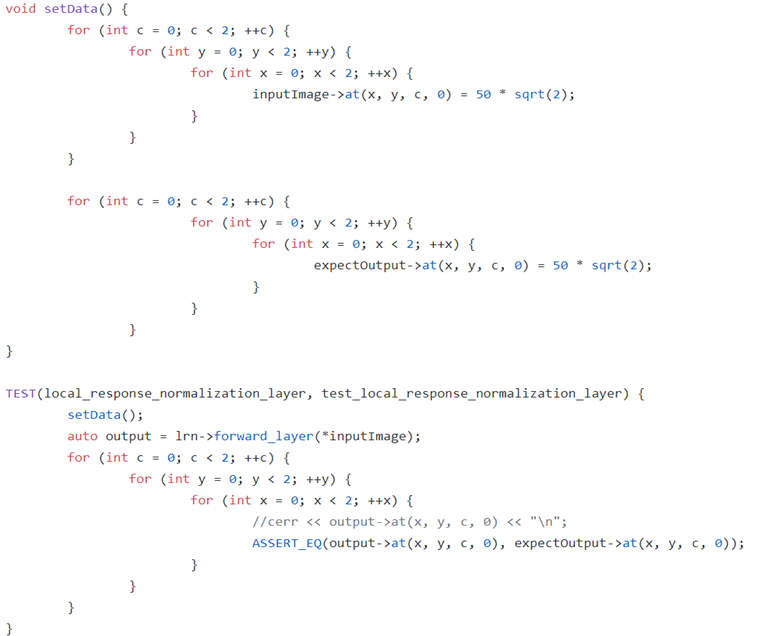
\includegraphics[width=1\textwidth]{local_response_test}
		\caption{local response test}
		\label{fig:local_response_test}
\end{figure}

\subsubsection{Fully Connected}
This layer basically takes an input volume (whatever the output is of the conv or ReLU or pool layer preceding it) and outputs an N dimensional vector where N is the number of classes that the program has to choose from.

After creating this objets and adding the data to each object we tested if the expected output is equals to the output of the connected layer with the assertion method. See \ref{fig:fully_connected_test} % insert here screenshot of test code

\begin{figure}[h]
		\centering
		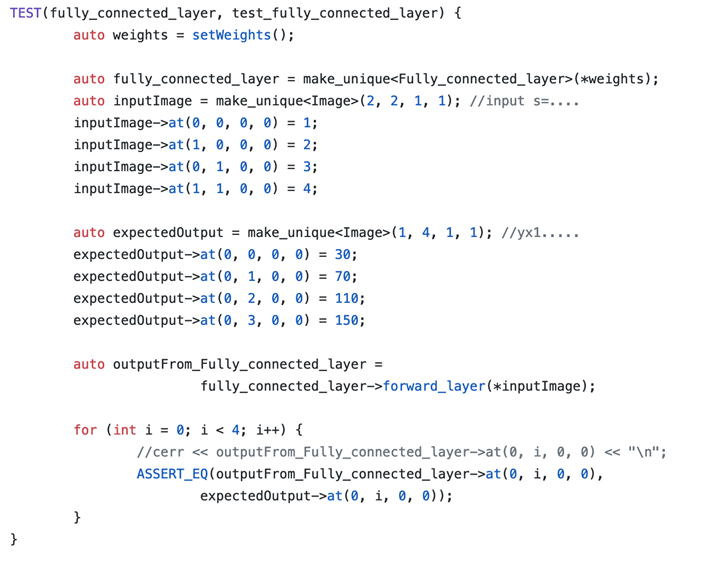
\includegraphics[width=1\textwidth]{fully_connected_test}
		\caption{fully connected test}
		\label{fig:fully_connected_test}
\end{figure}

\pagebreak
\subsection{Input Output Management}
These classes work directly with the user interface, and provide through it the input images and platforms, as well as the mode to the back end , and offer access to the results, whether seperately, or aggregated.
\subsubsection{Assistant}
The assistant has the input images stored in a map, with their respective paths. See \ref{fig:assistant_test} % insert here screenshot of test code

\begin{figure}[h]
		\centering
		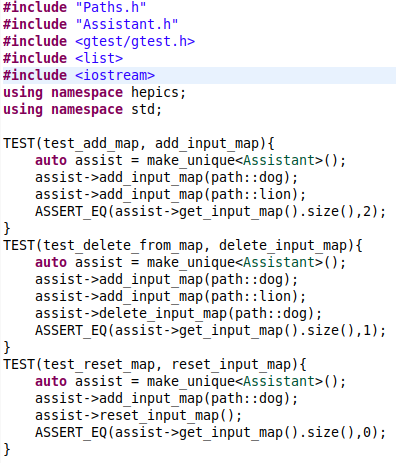
\includegraphics[width=0.55\textwidth]{assistant_test}
		\caption{assistant test}
		\label{fig:assistant_test}
\end{figure}


\subsubsection{Result}
This is a basic representation of the results stored in a vector of pairs, sorted descendently.
\subsubsection{DataSaver}
The datasaver saves outputs of the classification, converts them into result objects and saves them into a map, directly providing access to them. It also can aggregate the current stored results. See \ref{fig:data_saver_test} % insert here screenshot of test code

\begin{figure}[h]
		\centering
		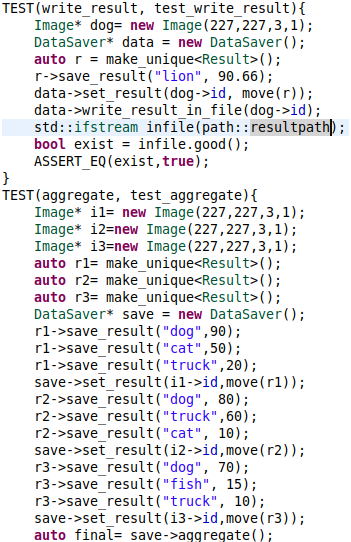
\includegraphics[width=0.46\textwidth]{data_saver_test}
		\caption{data saver test}
		\label{fig:data_saver_test}
\end{figure}

\subsubsection{Scheduler}
The scheduler is responsible of providing the system with information about platforms it can run on, depending on the user's choise of platforms and operation mode. See \ref{fig:scheduler_test} % insert here screenshot of test code

\begin{figure}[h]
		\centering
		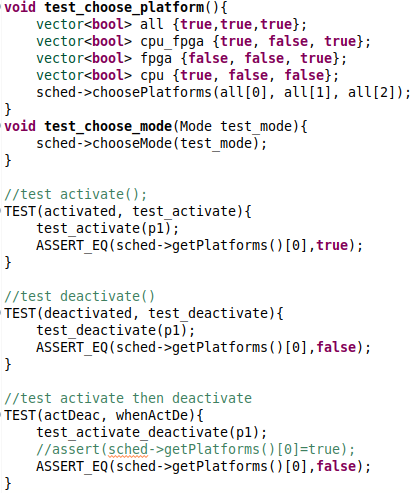
\includegraphics[width=0.54\textwidth]{scheduler_test}
		\caption{scheduler test}
		\label{fig:scheduler_test}
\end{figure}

\pagebreak
\subsection {Test results}
\begin{figure}[b]
\centering
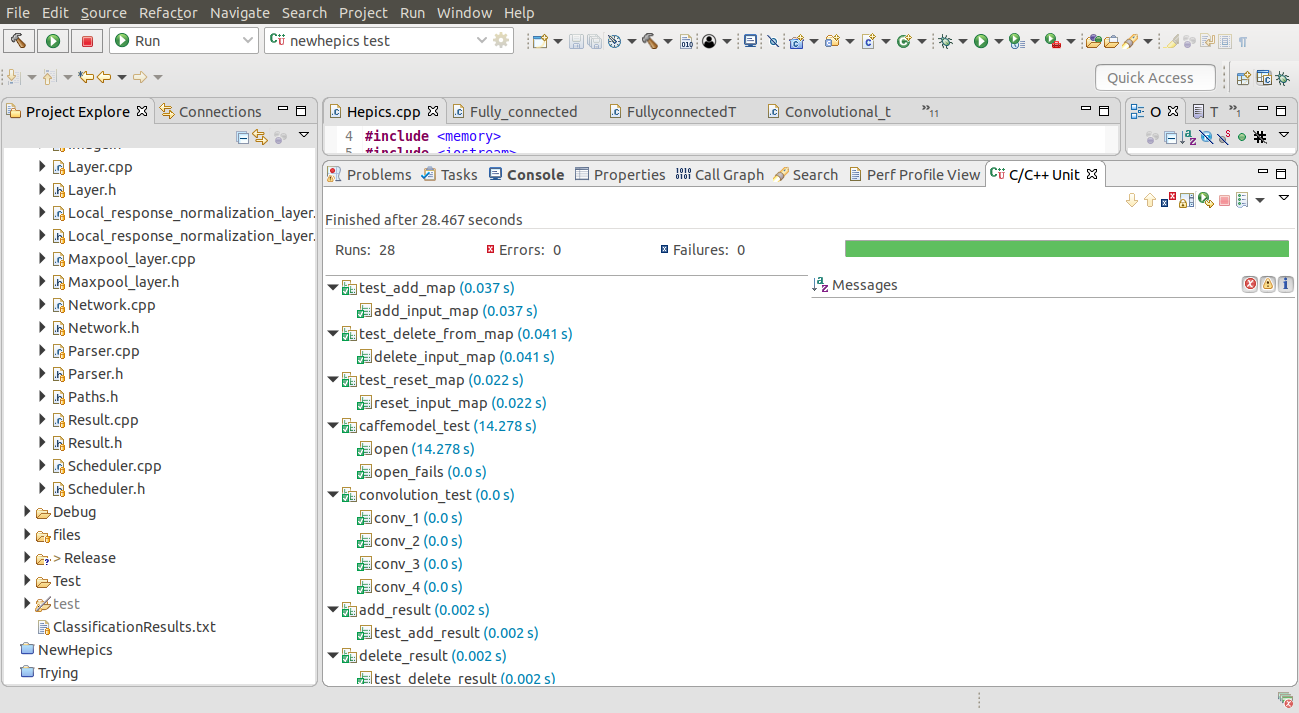
\includegraphics[width=0.45\textwidth, center]{test1}
\end{figure}
\begin{figure}[b]
\centering
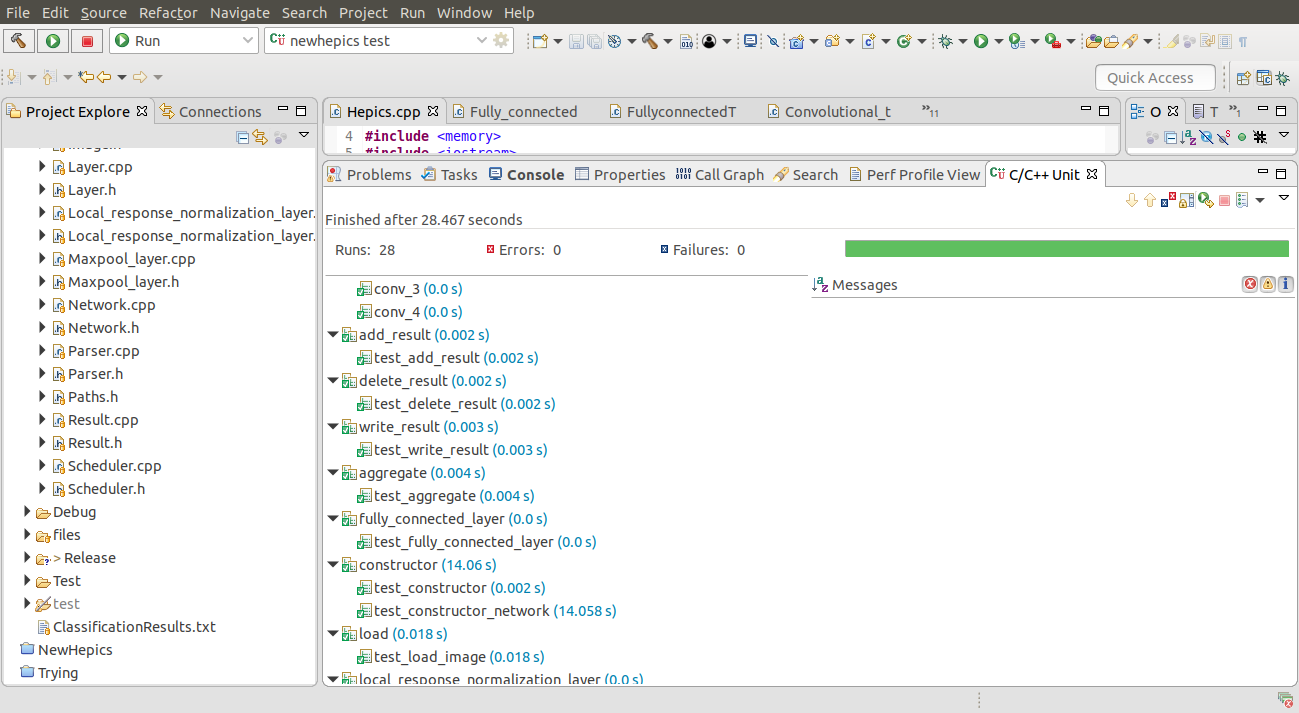
\includegraphics[width=0.45\textwidth, center]{test2}
\end{figure}
\begin{figure}[b]
\centering
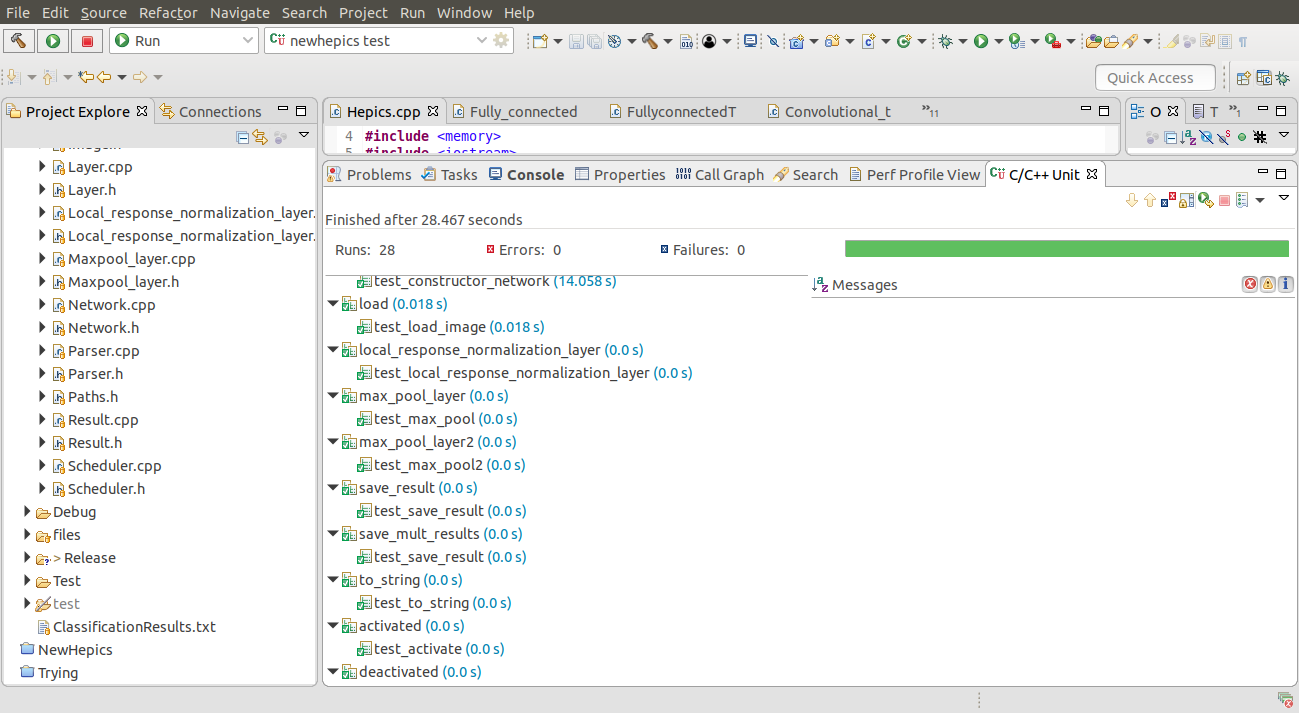
\includegraphics[width=0.45\textwidth, center]{test3}
\end{figure}
\begin{figure}[b]
\centering
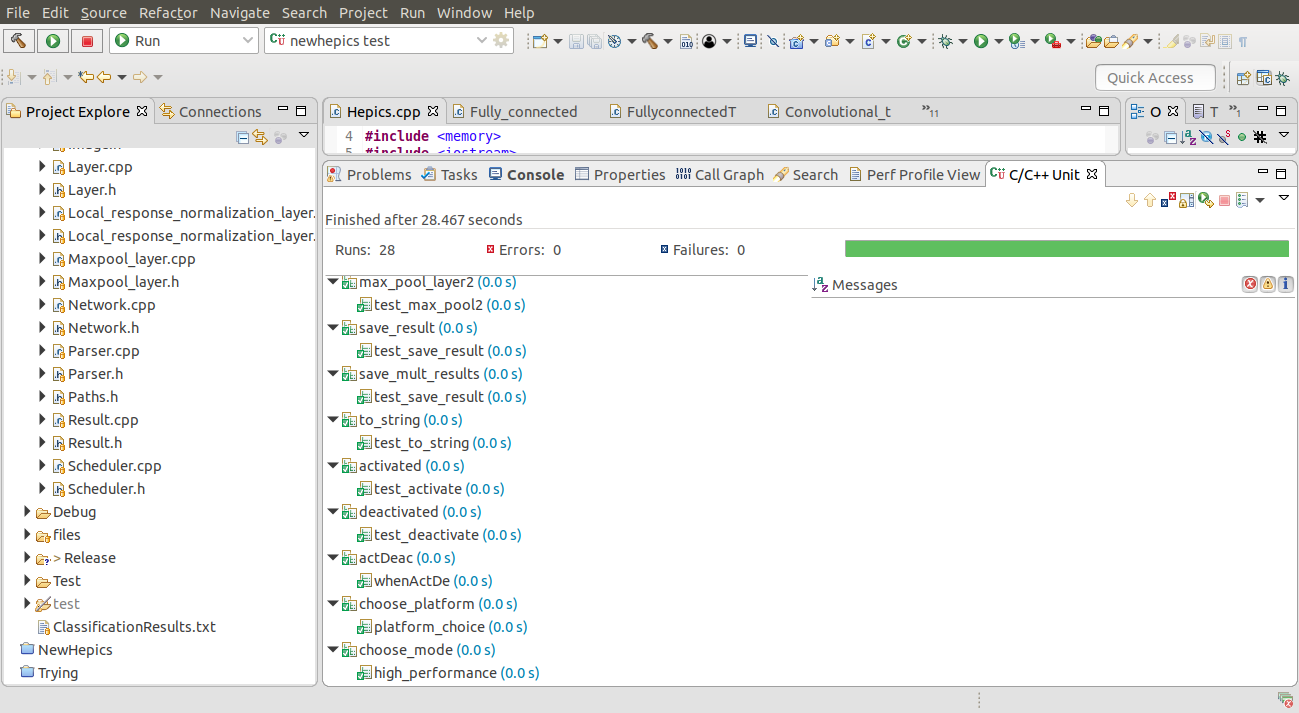
\includegraphics[width=0.45\textwidth, center]{test4}
\end{figure}


\pagebreak
\section {Coverage}
Gcov is a test coverage program. We used it in concert with GCC to analyze our programs and help create more efficient, faster running code, and discover untested parts of the program. Gcov is an efficient profiling tool to help discover where the optimization efforts will best affect the code.\\
Gcov profiling tools helped us analyze our code's performance. By using gcov we found some basic performance statistics, such as:
\begin{itemize}
	\item how often each line of code executes
	\item what lines of code are actually executed
	\item how much computing time each section of code uses
\end {itemize}


% insert here coverage screenshot
\pagebreak
\section {Current Overall State}
Eclipse CDT , which was used to manage the back-end build, and QtCreator ,which was used to manage the GUI build, are not especially set to work with each other, and use two different ways of building and compiling projects.
Since the classification is the core of this project, we opted to run both seperately until we manage to make both of the GUI and classification run on eclipse. We trust we have made a big step in this direction, since basic GUI's are now running on eclipse, however we still have compiling errors when merging both of the main projects.

\end{document}
